\documentclass[a4paper, DIV12, 2.5headlines, headings = big, titlepage, openbib]{scrartcl}

\usepackage[ngerman]{babel}
\usepackage[T1]{fontenc}
\usepackage{geometry}
\usepackage[utf8x]{inputenc}
\usepackage{mathpazo}
\usepackage{helvet}
\usepackage{courier}
\usepackage{eurosym}
\usepackage{amsmath}
\usepackage{courier}
\usepackage{scrpage2}
\usepackage{graphicx}
\usepackage{xcolor}
\usepackage{multirow}
\usepackage{varioref}
\usepackage{babelbib}
\usepackage{makeidx}
\usepackage{tabularx}
\usepackage{floatflt}
\usepackage{float}
\usepackage{lipsum}
\usepackage{xargs}
\usepackage{enumitem}
\usepackage{listings}
\usepackage{wrapfig}
\usepackage[colorinlistoftodos,prependcaption,textsize=tiny]{todonotes}
\usepackage[pdftex, colorlinks, linktocpage, linkcolor=black, citecolor=black, urlcolor=black]{hyperref}
\usepackage[linesnumbered]{algorithm2e}

\pagestyle{scrheadings}

\geometry{a4paper, top=55mm, left=40mm, right=35mm, bottom=40mm, headsep=10mm, footskip=22mm}
\linespread {1.25}

\newcommand{\theauthor}{Niklas Kiefer}
\newcommand{\matrnr}{775107}
\newcommand{\thetitle}{Providing a distributed file storage for German Schul-Cloud}
\newcommand{\thesubtitle}{Erstellung einer verteilten Dateiverwaltung für die deutsche Schul-Cloud}

\definecolor{code_background}{HTML}{F7F7F7}
\definecolor{code_frame}{HTML}{DDDDDD}
\definecolor{code_comments}{HTML}{969896}
\definecolor{code_keywords}{HTML}{A71D5D}
\definecolor{code_numbers}{HTML}{969896}
\definecolor{code_strings}{HTML}{183691}
\definecolor{code_identifiers}{HTML}{333333}
% Rot
\definecolor{hpired}{rgb}{0.686,0,0.204}
% Orange
\definecolor{hpiorange}{rgb}{0.867,0.380,0.031}	
% Gelb
\definecolor{hpiyellow}{rgb}{0.965,0.659,0}					%100 
\colorlet{hpiyellow2}{hpiyellow!60!white}					% 60
\colorlet{hpiyellow3}{hpiyellow!40!white}					% 40
\colorlet{hpiyellow4}{hpiyellow!20!white}					% 20
% Grau
\definecolor{hpigrey}{rgb}{0.376,0.408,0.420}				%100
\colorlet{hpigrey2}{hpigrey!70!white}						% 70
\colorlet{hpigrey3}{hpigrey!50!white}						% 50
\colorlet{hpigrey4}{hpigrey!20!white}						% 20
% Blau
\definecolor{hpiblue}{rgb}{0,0.478,0.620}					%100
\colorlet{hpiblue2}{hpiblue!60!white}						% 60
\colorlet{hpiblue3}{hpiblue!40!white}						% 40
\colorlet{hpiblue4}{hpiblue!15!white}						% 15
\usepackage{array}
\usepackage{supertabular}
\usepackage{colortbl}

% TODO
\newcommandx{\unsure}[2][1=]{\todo[linecolor=red,backgroundcolor=red!25,bordercolor=red,#1]{#2}}
\newcommandx{\change}[2][1=]{\todo[linecolor=blue,backgroundcolor=blue!25,bordercolor=blue,#1]{#2}}
\newcommandx{\info}[2][1=]{\todo[linecolor=green,backgroundcolor=green!25,bordercolor=green,#1]{#2}}
\newcommandx{\improvement}[2][1=]{\todo[linecolor=green,backgroundcolor=green!25,bordercolor=green,#1]{#2}}
\newcommandx{\thiswillnotshow}[2][1=]{\todo[disable,#1]{#2}}

\newcommand{\frontmatter}{\pagenumbering{roman}}
\newcommand{\mainmatter}{\pagenumbering{arabic}\setcounter{page}{1}}

\newcounter{todocounter}
\setcounter{todocounter}{0}
\newcounter{authcounter}
\setcounter{authcounter}{0}
%%% BEGIN Write TODO in File
\def\getdefhelp#1->#2\endhelp{#2}
\def\getdef#1#2{\edef#2{\expandafter\getdefhelp\meaning#1\endhelp}}
\newwrite\TodoDatei
\newwrite\AuthorDatei
\openout\AuthorDatei=author.out
\newcommand{\WriteTodo}[2]{%
	\def\Cont{#2}
	\getdef\Cont\Content
	\edef\WriteIndex{%
		\write\TodoDatei{\string\textcolor{#1}{\string\textbf{\Content}}\string\dotfill\string\pageref{todo:\thetodocounter}}}%
	\WriteIndex}

\newcommand{\WriteAuthor}[1]{%
	\def\Cont{#1}
	\getdef\Cont\Content
	\edef\WriteAuth{\write\AuthorDatei{\Content\string\dotfill\string\ref{auth:\theauthcounter}}}
	\WriteAuth}


%%% END Write TODO in File

% command \BibTeX
\def\BibTeX{{\rm B\kern-.05em{\sc i\kern-.025em b}\kern-.08em
     T\kern-.1667em\lower.7ex\hbox{E}\kern-.125emX}} 

% day in journal: \journalday{date}{titel}{persons}{aktivity}
\newcommand{\journalday}[4]{%
\def\titleTmp{#2}
\subsection*{#1\ifx\titleTmp\empty{}\else{: #2}\fi}
\begin{center}
\begin{tabularx}{\textwidth}{@{}lX@{}}
	Anwesende: & #3\\
	Vorgang: & #4
\end{tabularx}
\end{center}
}

% errorreport: \errorreport{date}{error}{reason}{solution}
\newcommand{\errorreport}[4]{%
\def\dateTmp{#1}
\def\errorTmp{#2}
\def\reasonTmp{#3}
\def\solutionTmp{#4}
\ifx\errorTmp\empty{}\else{%
\subsection*{\ifx\dateTmp\empty{}\else{\hfill(#1)\\}\fi Problem: #2}%
{\begin{center}%
\vskip-1ex%
\begin{tabularx}{\linewidth}{@{}lX@{}}
	Ursache: & \ifx\reasonTmp\empty{unbekannt}\else{#3}\fi\\
	L�sung: & \ifx\solutionTmp\empty{unbekannt}\else{#4}\fi\\
\end{tabularx}%
\end{center}%
}}\fi}

% code: \code[textcolor]{backgroundcolor}{content}
\newcommand{\code}[3][black]{%
	\begin{flushleft}	
		\ttfamily
		\small
		\fcolorbox{#1}{#2}{\textcolor{#1}{\shortstack[l]{#3}}}
	\end{flushleft}
}

% code with white borderline
\newcommand{\codeblank}[3][black]{%
	\begin{flushleft}	
		\ttfamily
		\small
		\fcolorbox{white}{#2}{\textcolor{#1}{\shortstack[l]{#3}}}
	\end{flushleft}
}

% centered code: \centercode[textcolor]{backgroundcolor}{content}
\newcommand{\centercode}[3][black]{%
	\begin{center}	
		\ttfamily
		\small
		\fcolorbox{#1}{#2}{\textcolor{#1}{\shortstack[l]{#3}}}
	\end{center}
}

% centered code with white borderline
\newcommand{\centercodeblank}[3][black]{%
	\begin{center}	
		\ttfamily
		\small
		\fcolorbox{white}{#2}{\textcolor{#1}{\shortstack[l]{#3}}}
	\end{center}
}


% annotation in colored box: \annot[text- and bordercolor]{backgroudcolor}{contents}
\newcommand{\annot}[3][black]{%
	\begin{center}	
		\fcolorbox{#1}{#2}{\textcolor{#1}{\shortstack[l]{\vspace*{1ex}\\\hspace*{.025\textwidth}\textbf{Anmerkung:}\\\hspace*{.05\textwidth}\parbox{.88\textwidth}{#3\vspace*{2ex}}\hspace*{.05\textwidth}}}}
	\end{center}
}

% annotation in colored box: \annot[text- and bordercolor]{backgroudcolor}{contents}
\newcommand{\hint}[3][black]{%
\begin{figure}[!t]
  \centering
  \fcolorbox{#1}{#2}{
    \begin{minipage}{.96\linewidth}
      \hspace*{.025\linewidth}\parbox{.93\linewidth}{\textbf{Hinweis:}}\hspace*{.025\linewidth}\\
      \hspace*{.05\linewidth }\parbox{.88\linewidth}{\vspace*{3ex}#3\vspace*{3ex}}\hspace*{.05\linewidth}
    \end{minipage}
  }
\end{figure}
}

\newcommand{\colorparbox}[3][.985\textwidth]{%
\begin{flushleft}
\fcolorbox{black}{#2}{\parbox{#1}{#3}}
\end{flushleft}
}

\newcounter{versionID}
\newenvironment{versioning}[1][hpiblue4]{%
\setcounter{versionID}{0}
\begin{center}	
	\tablefirsthead{%
		\hline
		\rowcolor{#1}
		\parbox[c][2em][c]{\linewidth}{\centering\textbf{lfd. Nr.}} &
		\parbox[c][2em][c]{\linewidth}{\centering\textbf{Bearbeiter}} & 
		\parbox[c][2em][c]{\linewidth}{\centering\textbf{�nderungen}}\\
		\hline}
	\tablehead{%
		\extrahead
		\hline
		\rowcolor{#1}
		\parbox[c][2em][c]{\linewidth}{\centering\textbf{lfd. Nr.}} &
		\parbox[c][2em][c]{\linewidth}{\centering\textbf{Bearbeiter}} & 
		\parbox[c][2em][c]{\linewidth}{\centering\textbf{�nderungen}}\\
		\hline}
	\tabletail{%
		\hline
		\multicolumn{3}{|r|}{\cellcolor{hpiblue4}\small\sl Fortsetzung auf der n�chsten Seite}\\
		\hline}
	\tablelasttail{}
	\begin{supertabular}{|p{.1\linewidth}|p{.25\linewidth}|p{.5\linewidth}|}
	}{%
	\end{supertabular}
\end{center}
\newwrite\VersionDatei
\openout\VersionDatei=theversion.aux
\write\VersionDatei{\theversionID}
\closeout\VersionDatei
%\vfill
}

\newcommand{\version}[2]{%
\parbox{\linewidth}{\centering\stepcounter{versionID}\theversionID} & 
\parbox[t]{\linewidth}{\centering#1} &
#2 \\\hline
}

\newcommand{\currentversion}[1][]{
\def\test{#1}
\def\drafttest{draft}
\def\finaltest{final}
\ifx\test\drafttest
	\def\versiontext{(Entwurf)}
\else
	\ifx\test\finaltest
		\def\versiontext{(Final)}
	\else
		\def\versiontext{}
	\fi
\fi
\vskip.3cm
\newread\DatenDatei
\openin\DatenDatei=theversion.aux
\ifeof\DatenDatei\def\curVers{---}\else\read\DatenDatei to \curVers\fi
\closein\DatenDatei
{\small Dokumentversion: \curVers{}\versiontext}}

%% Acceptance Criterions
\newenvironment{acceptance}[1][hpiblue4]{%
\begin{center}	
	\tablefirsthead{%
		\hline
		\multicolumn{2}{|l|}{\cellcolor{hpiblue3}\bfseries Abnahmekriterien:}\\
		\hline}
	\tablehead{%
		\hline
		\multicolumn{2}{|l|}{\cellcolor{hpiblue3}\bfseries Abnahmekriterien (Fortsetzung):}\\
		\hline}
	\tabletail{%
		\multicolumn{2}{|r|}{\cellcolor{hpiblue4}\small\sl Fortsetzung auf der n�chsten Seite}\\
		\hline}
	\tablelasttail{}
	\begin{supertabular}{p{.23\linewidth}p{.7\linewidth}}
	}{%
	\end{supertabular}
\end{center}
\vfill
}

\newcommand{\criterion}[3]{%
	& \\
	\rowcolor{hpiblue4}Ausgangssitiation: & #1 \\
	Ereignis: & #2 \\
	Erwartetes Ergebnis: & #3 \\
}

\newcommand{\authindex}[1]{\expandafter\index{#1}}
%% SecAuthor
\newcommand{\secauthor}[2]{%
\def\secChap{chapter}
\def\secSect{section}
\def\secSubs{subsection}
\edef\refer{#1!Abschnitt \thesection}
\def\sec{#2}
\ifx\sec\secChap\edef\refer{#1!Kapitel \thechapter}\fi
\ifx\sec\secSect\edef\refer{#1!Abschnitt \thesection}\fi
\ifx\sec\secSubs\edef\refer{#1!Abschnitt \thesubsection}\fi
\label{auth:\theauthcounter}
\authindex{\refer}
%In Datei schreiben
%\WriteAuthor{#2}
\stepcounter{authcounter}
}

\newif\ifnotdone

\newcommand{\readLine}[1]{%
\ifeof#1
	\def\tobedone{}
	\notdonefalse
\else
	\read\TodoFileIn to \tobedone
	\notdonetrue
\fi
\tobedone\par}

%%% XML-Command
\newdimen\LineFeedDim
\LineFeedDim = 1.5em
\newdimen\LineFeed
\newif\ifXMLintern

\newcommand{\Tag}[4][black]{%
\ifXMLintern\\\hskip\LineFeed\fi%
\XMLinternfalse%
\textcolor{#1}{<#2}%
\def\paratest{#3}%
\ifx\paratest\empty{}%
\else{} #3%
\fi%
\global\advance\LineFeed by \LineFeedDim%
\def\contenttest{#4}%
\ifx\contenttest\empty%
	\global\advance\LineFeed by -\LineFeedDim\textcolor{#1}{/>}%
\else%
\textcolor{#1}{>}\\\hskip\LineFeed#4\\%
\global\advance\LineFeed by -\LineFeedDim\ifdim\LineFeed > 0em\hskip\LineFeed\fi\textcolor{#1}{</#2>}%
\fi\XMLinterntrue%
}

%% <? ... ?> als Argument �bergeben -> processing, comment, normal
\def\proctest{processing}
\def\commtest{comment}
\def\normtest{normal}
\newcommand{\LineTag}[4][normal]{%
\ifXMLintern\\\hskip\LineFeed\fi%
\XMLinternfalse%
\def\argtest{#1}%
<\ifx\argtest\proctest ?\else\ifx\argtest\commtest !-- \fi\fi#2%
\def\partest{#3}%
\ifx\partest\empty%
\else{} %
	#3%
\fi%
\def\contenttest{#4}%
\ifx\contenttest\empty%
\def\argtest{#1}%
\ifx\argtest\proctest{} ?\else\ifx\argtest\commtest{} --\else/\fi\fi>%
\else> #4 </#2>\fi\XMLinterntrue%
}

\newcommand{\EmptyTag}[1][]{%
\ifXMLintern\\\hskip\LineFeed\fi#1\parbox[c][1ex][c]{1ex}{}\XMLinterntrue%
}

\newcommand{\NewLinePar}{%
\\\hskip\LineFeed\hskip3em
}

\newcommand{\xml}[3][black]{%
	\LineFeed=0em
	\XMLinternfalse
	\small
	\fcolorbox{#1}{#2}{\ttfamily\shortstack[l]{#3}}
}

\newcommand{\soapmsg}[7][hpigray4]{%
	{\centering
	\begin{tabularx}{\linewidth}{|l|X|}
		\hline
		\cellcolor{#1}K�rzel & #2 \\
		\hline
		\cellcolor{#1}Consumer & #3 \\
		\hline
		\cellcolor{#1}Request Parameter & #4 \\
		\hline
		\cellcolor{#1}Response Parameter & #5 \\
		\hline
		\cellcolor{#1}Kurzbeschreibung & #6 \\
		\hline%
		\cellcolor{#1}Doppelter Request & #7 \\
		\hline
	\end{tabularx}
	}
}

\newcommand{\myabstract}[2]{%
	\def\germtest{#1}
	\def\engltest{#2}
	\ifx\germtest\empty
		\ifx\engltest\empty
		\else
			\hbox{ }
			\vfill
		\fi
	\else
		%\hbox{ }
		%\vfill
  \fi
	\ifx\germtest\empty\else
  	\begin{quotation}
  	\begin{center}\normalfont\sectfont\nobreak Kurzfassung\end{center}
  	#1
  	\end{quotation}
  	\vskip1cm
  	\clearpage
  \fi
  \ifx\engltest\empty\else
  	\begin{quotation}
  	\begin{center}\normalfont\sectfont\nobreak Abstract\end{center}
  	#2
  	\end{quotation}
	\fi
	\ifx\germtest\empty
		\ifx\engltest\empty
		\else
  		\vfill
  		\vfill
  		\clearpage
		\fi
	\else
  	\vfill
  	\vfill
  	\clearpage
  \fi
}
% Eigene Umgebungen
\newenvironment{otherenumi}[1]{%
	\renewcommand*{\labelenumi}{#1}
	\begin{enumerate}
	}{%
	\end{enumerate}
	\renewcommand*{\labelenumi}{\alph{enumi})}}
\newenvironment{otherenumii}[1]{%
	\renewcommand*{\labelenumii}{#1}
	\begin{enumerate}
	}{%
	\end{enumerate}
	\renewcommand*{\labelenumi}{\alph{enumi})}}


\lstdefinestyle{JavaScript}{
    backgroundcolor=\color{code_background},
    commentstyle=\color{code_comments},
    keywordstyle=\color{code_keywords},
    numberstyle=\tiny\color{code_numbers},
    stringstyle=\color{code_strings},
    identifierstyle=\color{code_identifiers},
    basicstyle=\scriptsize,
    aboveskip=5mm,
    belowskip=5mm,
    xleftmargin=0mm,
    xrightmargin=-20mm,
    breakatwhitespace=false,
    breaklines=true,
    captionpos=b,
    keepspaces=true,
    numbers=left,
    numbersep=10pt,
    frameround=ftff,
    frame=single,
    rulecolor=\color{code_frame},
    showspaces=false,
    showstringspaces=false,
    showtabs=false,
    tabsize=2
}
\lstset{style=JavaScript}
\lstMakeShortInline[
	columns=fixed,
	basicstyle=\ttfamily
]|

\setlength{\parindent}{0cm}
\setlength{\parskip}{0.25cm}

\begin{document}

	%%% Headers & Footers
	\selectlanguage{ngerman}
	\automark{section}
	\ohead{
\includegraphics[height=1.3cm,clip,viewport={0 60 250 180}]{utils/hpi_logo.pdf}}
	\chead{}
	\ihead{\headmark}
	\setheadsepline{1.0pt}[\color{hpigrey}]

	%%% Title page
	\hypersetup{%
		pdftitle	= {\thetitle},
		pdfsubject	= {Bachelor Thesis},
		pdfauthor	= {\theauthor},
		pdfcreator	= {PDFLaTeX},
		pdfproducer	= {LaTeX with hyperref and thumbpdf}
	}

	\titlehead{
	\centering
	
\includegraphics[height=4cm]{utils/hpi_logo.jpg}
}
\subject{{\LARGE Bachelor's Thesis}\\}
\title{\thetitle}
\subtitle{\thesubtitle}
\author{{\small by}\\\textbf{\theauthor}}
\date{Potsdam, June 2017}
\publishers{
	\textbf{Supervisor}\\
	\vskip1em
	Prof. Dr. Christoph Meinel,\\
	Jan Renz\\

	\vskip1em
	\textbf{Internet-Technologies and Systems Group}
}
\frontmatter
\maketitle


	%%% Disclaimer
	\section*{Disclaimer}

Hiermit versichere ich, dass diese Arbeit selbst\"{a}ndig verfasst wurde und dass keine anderen Quellen und Hilfsmittel als die angegebenen benutzt wurden. Diese Aussage trifft auch f\"{u}r alle Implementierungen und Dokumentationen im Rahmen dieses Projektes zu. \\\\
I certify that the material contained in this dissertation is my own work and does not contain significant portions of unreferenced or unacknowledged material. I also warrant that the above statement applies to the implementation of the project and all associated documentation.

\begin{flushleft}
	Potsdam, \today
\end{flushleft}
\begin{picture}(150,70)
	\put(0,15){\line(1,0){150}}
	\put(0,0){(\theauthor)}
\end{picture}

\clearpage

	%%% Abstract
	%%\myabstract{
	
	
	
}

	%%% TOC
	\tableofcontents
	\clearpage

	\mainmatter
	%% Content
	\section{Einleitung}
\label{sec:intro}

Die deutsche Schul-Cloud soll ``dabei helfen, die digitale Transformation in Schulen zu meistern und den fächerübergreifenden Unterricht mit digitalen Inhalten zu bereichern'' \footnote{ Technischer Bericht (Seite 5) \cite{paper:technischerbericht}}. Ein Schwerpunkt ist hierbei das Arbeiten mit verschiedenen Dateiformaten im Unterrichtskontext. Dazu soll die Schul-Cloud eine Möglichkeit schaffen, eigene Dateien zu verwalten und sie unter Lehrern und Schülern zu teilen. Die Bildung einer Dateiablage ist nach neueren Analysen fester Bestandteil von ``technisch-organisatorische Kernanforderungen" \cite{paper:breiterstolpmannzeising2015} für den digitalen Unterricht. Dafür soll keine neue Dateiverwaltungstechnologie entworfen werden, sondern auf bestehende Systeme zurückgegriffen werden. Vielmehr soll es für den Nutzer der Schul-Cloud möglich sein, ein bestehende Dateiablage weiter zu nutzen und in die Schul-Cloud zu integrieren. Außerdem ist es erforderlich, Dateien auf verschiedenen Systemen zu lagern, um eine flexible Architektur zu schaffen. Dies ist vor allem dann nötig, wenn große Datenmengen von sehr vielen Schulen, Schülern und Lehrern entstehen. Dann ist es wichtig, eine Lösung in Form eines verteilten File Storage zu finden. 

In dieser Bachelor-Arbeit wird eine solche Architektur für ein verteiltes Dateiverwaltungssystem beschrieben und entworfen. Begonnen wird mit einer \textbf{Vorbetrachtung} (2), in welcher die bestehende Situation von Dateiverwaltung im Schulunterricht diskutiert wird. Auch werden bereits bestehende Konzepte anderer Arbeiten analysiert und Vorbilder ausgemacht. Danach wird ein \textbf{Konzept} (3) für ein verteiltes System beschrieben und anschließend eine mögliche \textbf{Implementierung} (4)  aufgezeigt. In dieser wird eine Anbindung von File Storage-Providern im Schul-Cloud Server und Client beschrieben. Diese Anbindungsmöglichkeit wird anschließend \textbf{evaluiert} und mögliche \textbf{Anschlussszenarien} aufgezeigt (5). Zum Ende werden die Ergebnisse \textbf{zusammengefasst} (6).

\clearpage

	\section{Vorbetrachtung und Verwandte Arbeiten}
\label{sec:relatedwork}

Als erstes gilt es, gegenwärtige Technologien zu evaluieren, um eine solide Grundlage für eine verteilte Dateiverwaltung für die Schul-Cloud zu erstellen. Wie in der Einleitung erwähnt wurde, soll kein neuartiges Dateiverwaltungskonzept geschaffen werden. Vielmehr soll auf bestehenden Systemen und Technologien aufgebaut werden und deren Vorteile genutzt werden. Zu Beginn werden im Vorfeld formulierte Anforderungen aufgegriffen und analysiert. Hierzu diente der Technischen Bericht der Schul-Cloud \cite{paper:technischerbericht} als Grundlage, welcher in Zusammenarbeit des Hasso-Plattner-Instut mit dem Mint-EC enstand. Ebenfalls werden andere Konzepte zur Dateiverwaltung im Schul-Kontext durchsichtet und analysiert. Es schließt sich eine Beobachtung an, inwieweit Dateiablagen auf Basis von Cloud-Storage Providern bereits im Unterricht genutzt werden. Für eine abschließende Vorbetrachtung eignet sich eine Betrachtung bereits bestehender Cloud-Storage Anbieter, welche sich in der Praxis bewährt haben und weiträumigen Einsatz finden.

\subsection{Anforderungen an die Dateiverwaltung der Schul-Cloud}

\subsubsection{Die Cloud für Schulen in Deutschland: Konzept und Pilotierung der Schul-Cloud}

Der Technische Bericht der Schul-Cloud \cite{paper:technischerbericht} von (Meinel et. al) wurde von Wissenschaftlern am Hasso-Plattner-Institut in Potsdam geschrieben und beschäftigt sich mit einer ersten technischen Konzeption der Schul-Cloud. Dieser bildet die Grundlage für das Bachelor-Projekt der Schul-Cloud im Wintersemester 2016/17 und Sommersemester 2017, wessen sich diese Arbeit anschließt. Der Bericht beinhaltet im Kapitel 4.5 auch ein Konzept für das Dateimanagement. Dort wird beschrieben, dass Dateien auf allen Endgeräten verfügbar sein sollen. Außerdem wird ein Aufbau skizziert, auf den im weiteren Verlauf dieser Arbeit eingegangen wird (Kapitel 3). Weitere wichtige Aufgaben der Dateiverwaltung sollen das Speichern von ``zusätzlichen Metadaten, die Erzeugung von Thumbnails und die Verwaltung von Berechtigungen" \cite{paper:technischerbericht} sowie das Teilen von Inhalten sein.

\subsubsection{Studie „Bildung 2.0 - Digitale Medien in Schulen“}

Sinnbildlich für viele Studien im Bereich digitaler Bildung, zeigt dieser Bericht der BITKOM \cite{paper:studiebildung20} auf, dass die Bereitschaft von Schülern und Schülerinnen, von physischen zu digitalen Lerninhalten stetig wachse. Immer öfter diene ein Computer als Hilfe für die Bearbeitung von Hausaufgaben. Dies Zeigt auch die Abbildung 1. Auch kämen PCs öfter im Unterricht zum Einsatz. Allerdings würde die Qualität der IT-Infrastruktur nicht immer als positiv wahrgenommen. Der Wunsch nach besserer Ausstattung und intensiverem Nutzen von elektronischen Medien sei klar ersichtlich. Somit scheint eine Verbindung der Dateiverwaltung der Schul-Cloud mit dem Hausaufgaben - Dienst und Kursen sowie Fächern äußert sinnvoll, weshalb sich in dieser Arbeit vermehrt darauf bezogen wird.

\begin{figure}[H]
	\centering
	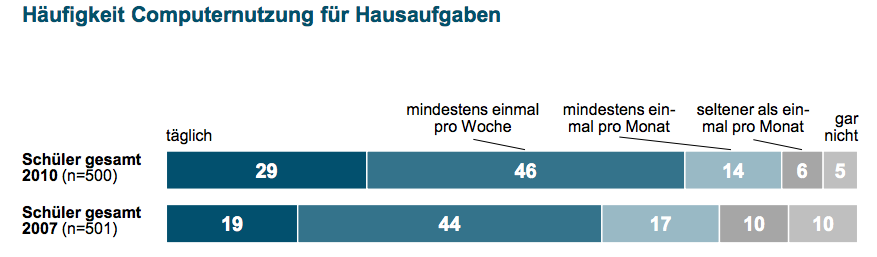
\includegraphics[width=0.8\linewidth]{images/BitkomNutzungComputerStudie}
	\caption[Caption for relatedWork]{Häufigkeit der Computernutzung für Hausaufgaben im Vergleich von 2007 zu 2010\footnotemark}
	\label{fig:BitkomNutzungComputerStudie}
\end{figure}
\footnotetext{Studie „Bildung 2.0 - Digitale Medien in Schulen“ (Folie 14) \cite{paper:studiebildung20}}

\subsubsection{Conceptual Architecture Design and Configuration of a Peer to Peer File System for Schools and Medium Sized Business}

Damian Clarke evaluierte in seinem Paper den Einsatz eines verteilten Dateisystem für Schulen und kleine Firmen \cite{paper:p2pfilesystemclarke}. Die Idee ist es, weg von einem üblichen zentralen Dateiserver zu einem verteilten Peer-to-Peer \footnote{Peer-to-Peer, eine gleichgestellte Rechner-zu-Rechner - Verbindung - \url{https://de.wikipedia.org/wiki/Peer-to-Peer}} zu wechseln, um so eine bessere Auslastung und ein skalierbares System zu erzielen. Gerade in der Schullandschaft sei es von Vorteil, auf eine verteilte Struktur zu setzen, da die Masse an Daten stetig zu nähme und die Kosten für Wartung und Erweiterung auf mehrere Träger besser zu verteilen wären. Dies ist besonders wichtig im Hinblick auf die Masse an Schulen in der Schul-Cloud. Wo zu Beginn noch 26 Partner-Schulen auf dem Produktivsystem unterwegs sind, werden dies mit Ausweitung nach der Pilotphase immer mehr. Somit macht eine Verteilung der Dateibestände auf mehrere Server Sinn.

\subsection{Nutzung von Cloud-Storage Providern im Unterricht}


Die Verwaltung von eigenen und geteilten Dateien wird mit der zunehmenden Digitalisierung des Unterrichts immer wichtiger. Wo es früher reichte, seine Unterrichtsmaterialien in einem Schulhefter zu legen, will man Arbeitsblätter und Wissenstexte heute überall und immer verfügbar haben. Um einen Eindruck in diese Problematik zu bekommen, wurde eine Umfrage zum Thema 'Dateiorganisation in der Schule' \cite{survey:umfragedateiorganisation} erstellt und an ehemaligen und aktuellen Schülern sowie Lehrern geschickt. Insgesamt nahmen \textbf{\textit{65}} \todo{Anpassen} Teilnehmer  an dieser Umfrage teil. Gefragt wurde unter anderem nach der Rolle des Teilnehmers (Schüler oder Lehrer) gefragt (Frage 1). Dabei sollten ehemalige Schüler und Lehrer vergangene Erfahrungen in die Beantwortung der Frage einfließen lassen. Dann wurde danach gefragt, ob der Befragte webbasierte Anwendungen zur Verwaltung der Dateien im Schulalltag benutzt hat (Frage 2). Anschließend wurde die Befragung geteilt. Wenn die Frage 2 mit 'Nein' beantwortet wurde, wurde nach Gründen für das Nichtbenutzen gefragt (Frage 3). Wurde Frage 2 mit 'Ja' beantwortet, wurde nach Vorteilen der Nutzung gefragt (Frage 4), sowie nach Beispielen, welche Dienste genutzt wurden (Frage 5). 

Die Ergebnisse \cite{survey:umfragedateiorganisationergebnisse} dieser Umfrage zeigen, dass eine Mehrheit der Befragten (ca. 72\%) auf solche Anbieter in ihrem Schulalltag verzichtet haben. Ein Großteil dieser Mehrheit gab an, dass Datenschutz ein großes Problem dabei darstellte. Ausländische Anbieter wie Dropbox \footnote{Dropbox - \url{https://www.dropbox.com/de/?landing=cntl}} oder Google Drive \footnote{Google Drive - \url{https://www.google.com/intl/de_ALL/drive/}} werden im pädagogischen Bereich eher kritisch betrachtet, da sie nicht in Deutschland gehostet werden und somit keine Transparenz in der Weiternutzung anfallender Daten erfolgt. Auch sind solche Dienste in Lernplattformen eher verpönt, da ``Schulen keinen Einfluss auf die Verwendung und Weiternutzung der hier anfallenden Daten und haben keine Vertragsbeziehung mit dem Betreiber dieser Dienste" \cite{online:itslearningmythenundfakten} haben. Weitere Gründe für die Nichtnutzung sind unter anderem, dass weite Teile des Unterrichtsmaterials offline zur Verfügung stehen, wie zum Beispiel einfache Arbeitsblätter, welche gar nicht erst digitalisiert werden. Oft ist auch einfach die Bereitschaft auf Seiten von Lehrer und Schüler gar nicht vorhanden, ihre Dateien online verfügbar zu machen, da die Ausstattung an den Schulen ohnehin auf einen weniger digitalen Unterricht ausgerichtet ist. Dazu kommen veraltete Technologien und schnelles Internet. Somit besteht auch kein Interesse daran, diese Dateien nur für den Gebrauch zu Hause verfügbar zu machen. Wenn dann doch Dateien von zu Hause in die Schule gebracht werden müssen, zum Beispiel Präsentationen oder Videos, wurden diese einfach auf einem USB-Stick gelagert.

Ein kleiner Teil der Befragten (ca. 28 \%) nutzten oder nutzen dagegen bereits Cloud-Storage Dienste für ihre Dateiverwaltung. Als meistgenutzter Dienst wurden hier Google Drive, One Drive  \footnote{One Drive - \url{https://onedrive.live.com/}} und Dropbox genannt. Ein sehr kleiner Teil benutzte sogar selbstgehostete Dienste wie zum Beispiel eine ownCloud \footnote{ownCloud - \url{https://owncloud.org/}}. Die Gründe hierfür seien die stetige Verfügbarkeit von mehreren Geräten, die papierlose Nutzung von Unterrichtsmaterialien, ein leichterer Backup von wichtigen Dateien und das Teilen mit mehren Personen. 

Die Auswertung der Umfrage zeigt, dass bei einem Großteil die Nutzung von cloudbasierten File-Storage Diensten eher auf Kritik stößt, als sie wirklich genutzt werden. Vor allem sind Datenschutz und schlechter Umgang mit digitalen Medien im Unterricht die Gründe hierfür. Mit einer einfachen Lösung innerhalb der Schul-Cloud, schnell an nötige Dateien für den Unterricht oder Hausaufgaben in digitaler Form zu kommen, könnte man hier ein Umdenken umleiten und die Vorteile sichtbar machen.

\subsection{Bestehende Cloud-Storage Provider}

Die Dateiverwaltung der Schul-Cloud soll nicht konzeptionell von Grund auf neu erstellt werden. Vielmehr soll auf bereits gut funktionierende und weit verbreitete Dienste zurückgegriffen werden. Auch soll es möglich sein, dass eine Schule selbst die Art des Hostings übernehmen kann, somit muss die Dateiverwaltung mehrere Typen einbinden können. Dies wird im Kapitel 3 als Form des Strategy-Patterns eingeführt, wodurch es möglich ist, Adapter für bestehende Anbieter zu schreiben. Im Folgenden werden solche Anbieter betrachtet, welche als erstes in die Schul-Cloud integriert wurden und werden sollen.

\subsubsection{AWS S3}

Als Teil der im Jahre 2006 eingeführten Amazon Web Services \footnote{Amazon Web Services - \url{https://aws.amazon.com/de/}} (AWS) bietet Amazon S3 (Simple Storage Service) als skalierbares Speichersystem zur Verfügung. S3 tritt hierbei als cloudbasierter Objektspeicher auf, der auf \textit{Buckets} und \textit{Objects} als Grundeinheiten basiert. Ein Bucket dient als einer Art Container, in dem mehrere Objects abgelegt werden. Ein Object ist somit eine Datei, die über einen \textit{Key} eindeutig in einem Bucket referenziert ist. In diesen Keys spiegelt sich auch die Ordnerstruktur innerhalb eines Bucket bzw. einen S3-Servers wieder. Dieser Aufbau wird als Quasi-Standard innerhalb von Storage Providern etabliert, wodurch sich die Dateiverwaltung der Schul-Cloud diesen Standard zu Nutze machen kann.

\subsubsection{ownCloud}

\subsubsection{Dropbox}

\todo[inline]{Zwar aus Datenschutz-Gründen nicht als Adapter vorgesehen, aber vom UI her vorbildhaft.}

\clearpage

	\section{Konzept}
\label{sec:concept}

In den vorangegangenen Kapiteln wurde aufgezeigt, was die Dateiverwaltung der Schul-Cloud leisten muss und woran sie sich orientieren kann. Vom Partner des Bachelor-Projekts MINT-EC \footnote{Verein mathematisch-naturwissenschaftlicher Excellence-Center an Schulen e. V. (MINT-EC) - \url{https://www.mint-ec.de/}}  und dem Hasso-Plattner-Institut wurde eine Anforderungsspezifikation erstellt, an welcher sich das folgende Konzept der Dateiverwaltung orientiert (Abbildung \ref{fig:anforderungen}). Neben der Verwaltung von eigenen Dateien, sollen auch  jene im Kurs- bzw. Fächer- so wie Klassenkontext verteilbar sein. Dies soll dazu dienen, digitale Inhalte besser in den Unterricht einzubetten und (Haus)-Aufgaben mithilfe von anschaulichem Material zu gestalten. Somit sollen diese Dateien über eine einheitliche Schnittstelle durch die Backend-API sowie über das Web-Frontend in mehreren Kontexten verfügbar sein. Außerdem soll es für eine Schule möglich sein, eine bereits bestehende Dateiablage einzubinden. 

\begin{figure}[H]
	\centering
	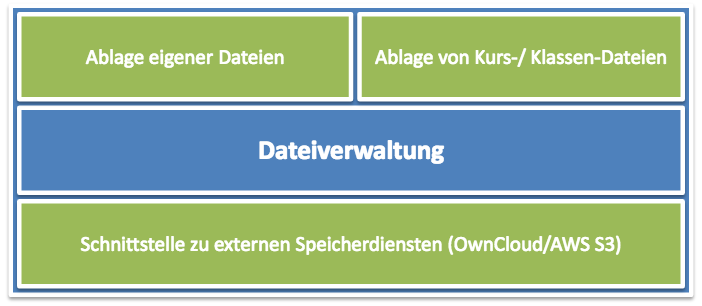
\includegraphics[width=0.8\linewidth]{images/AnforderungenDateiverwaltung}
	\caption[Caption for concept]{Grundanforderungen an die Dateiverwaltung der Schul-Cloud\footnotemark}
	\label{fig:anforderungen}
\end{figure}
\footnotetext{Martin Hense (Mint-EC - \url{https://www.mint-ec.de/})}


\subsection{Grundaufbau Dateiverwaltung}
\label{sec:basicaufbau}

Die grundlegende Struktur sieht vor, dass jede Schule seine eigene logische Einheit besitzt. Diese wird im folgenden \textit{Bucket} genant und leitet sich von der AWS S3-Nomenklatur ab (Abschnitt \ref{sec:awss3related}). Das dient zum einen der besseren Organisation innerhalb der Schul-Cloud, da Nutzer im Datenmodell zu einer Schule zusammengefasst werden. Außerdem folgt das Projekt dem Prinzip \textit{Privacy by Design} \footnote{Privacy by Design - \url{https://digitalcourage.de/blog/2015/was-ist-privacy-design} }. Damit wird sichergestellt, dass eine Schule von anderen modular abgekapselt wird. Somit ist von vornherein  eine Sicherheit der Dateien auf Schulebene gewährleistet. Diese Schul-Buckets können auf getrennten Servern liegen, so dass zum Beispiel eine Schule aus Niedersachsen auf eine eigene ownCloud zurückgreifen und eine Schule aus Hamburg einen S3-Provider benutzen kann. Das Prinzip des \textit{File Sharing} (Abschnitt \ref{sec:sharing_concept}) kann diese logische Abkapselung ein wenig aufbrechen, um Dateien auch über Schulebene hinaus teilbar zu machen. Eine Erweiterung von Buckets auf Landkreis - oder Bundeslandebene erscheint als weitere Option. Jedoch wird sich diese Arbeit auf die Einteilung in Schul-Buckets beschränken. Dieses Konzept ist aber ohne weiteres skalierbar auf größere Kontexte.  Die Abbildung \ref{fig:aufbau} zeigt im folgenden die weitere Unterteilung eines Buckets. Dieser wird in vier Teilkomponenten innerhalb der Schule  untergliedert. Wenn ein Bucket als einer Art Oberordner oder Root-Verzeichnis verstanden werden kann, dann sind diese Teilkomponenten schlichtweg Unterordner des Buckets. Zum einen gibt es den Ordner \textit{courses}, dieser enthält alle Dateien, welche zu Kursen bzw. Fächer gehören. Für eine bessere Unterteilung befinden sich hier sehr viele Unterordner, welche bloß die \textit{courseId} eines Schul-Cloud Kurses referenzieren. Dies dient der Verteilung aller Kurs-Dateien zu dem zugehörigen Kurs. Diese ID-Ordnernamen werden von Schul-Cloud Server versteckt und nicht im User Interface des  Clients angezeigt. So hat man aber zum Beispiel die Möglichkeit, über die \textit{courseId} alle Dateien eines Kurses zu erhalten. Auf diese haben nur Lehrer und Schüler des Kurses bzw. Faches Zugriff. Die Berechtigungsverwaltung übernimmt der Schul-Cloud Server und wird in der Implementierung (Abschnitt \ref{sec:permissionsimpl}) genauer beschrieben. \\

Ähnlich wie der \textit{courses} Unterordner gibt es den \textit{classes} und \textit{users} Unterordner. Beim ersten werden im gleichen Schema alle Dateien von Schul-Cloud Klassen verteilt, wieder referenziert über den jeweiligen ID-Unterordner. Zugriff haben hier nur Lehrer und Schüler der Klasse. Der \textit{users} Unterordner bildet die persönlichen Dateien eines jeden Nutzers der Schule, egal ob Lehrer, Schüler oder Administrator. Als Zusatz für schulübergreifende Dateien gibt es den Unterordner \textit{school}. Schreibrechte hat hier nur der Administrator der Schule, zugreifen kann jedoch jeder Nutzer der Schule. Natürlich kann es nun vorkommen, dass eine Schule bereits eine ausgeprägte Dateistruktur besitzt und der Grundaufbau mit den vier Unterkomponenten nicht abbildbar sein könnte. Hier muss der Schul-Cloud Server dafür sorgen, dass diese Dateien trotzdem über die Schul-Cloud zugänglich sind. Eine Möglichkeit wäre es, dass die gesamte Struktur zu Beginn in den \textit{schools} Ordner gelegt wird und diese von dahin auf die jeweiligen Kontexte verlegt werden.

\begin{figure}[H]
	\centering
	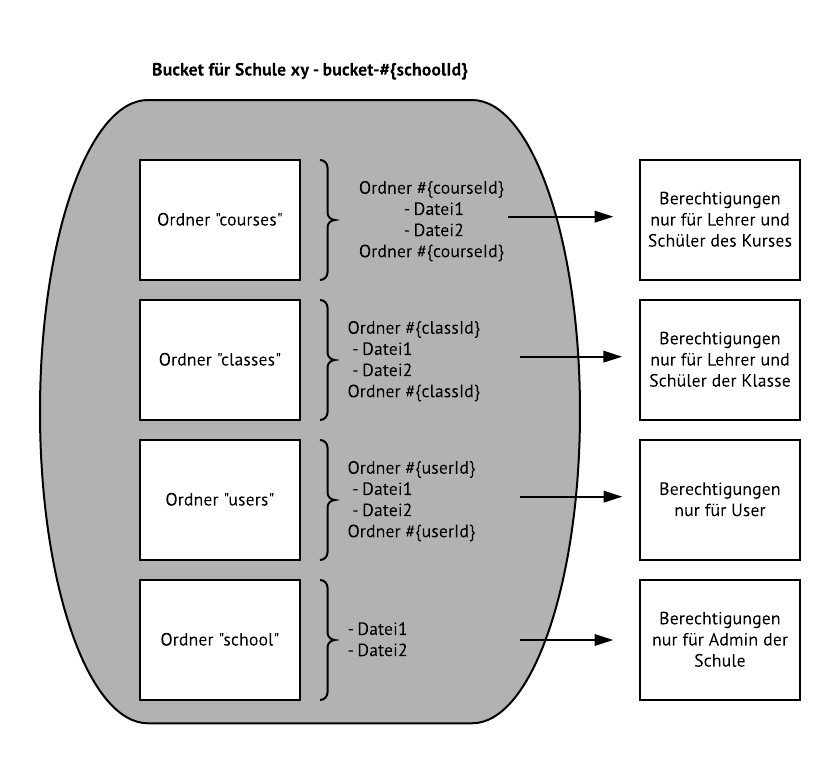
\includegraphics[width=0.8\linewidth]{images/AufbauDateiverwaltung}
	\caption[Caption for concept]{Grundaufbau eines Schul-Buckets}
	\label{fig:aufbau}
\end{figure}

\subsection{Architektur verteilter Provider}
\label{sec:strategypatternconcept}

Die Schul-Cloud stellt während der Pilotphase zwar nur eine S3-Instanz \footnote{Technischer Bericht der Schul-Cloud, Seite 39 \cite{paper:technischerbericht}}, worauf die Buckets der Pilotschulen liegen. Trotzdem soll es die Architektur der Dateiverwaltung möglich machen, Buckets auch auf mehrere Server zu verteilen. Dafür macht sich der Server das Strategy-Pattern \footnote{Strategy-Pattern - \url{https://de.wikipedia.org/wiki/Strategie_(Entwurfsmuster)}} zu Nutze. Dieses sieht vor, dass eine abstrakte Strategie die Schnittstellen vorgibt und mehrere Strategien diese implementieren. In Form dieser können so Anbindungen an verschiedene Typen von File Storage Providern erstellt werden. In der Implementierung wird eine solche Strategie am Beispiel von AWS S3 (Abschnitt \ref{sec:awss3impl}) geschildert. Abbildung \ref{fig:strategy} zeigt die Verteilung der verschiedenen File Storage Strategien. So ist es möglich, über den Schul-Kontext, der die Art des Provider bestimmt, die richtige Strategie zu bestimmen und auf die Schuldateien zugreifen zu können. Diese Aufteilung macht die Verteilung von Buckets auf mehrere Server ausführbar. So kann ein Bucket auf einer S3-Instanz liegen und mittels S3-Strategie darauf zugegriffen werden, sowie eine ownCloud-Instanz durch die ownCloud-Strategie auf einem anderen Server. Zwar ähnelt die genannte Struktur sehr dem S3-Ansatz, er lässt sich jedoch auch auf andere Typen einsetzen. Ein Bucket im ownCloud-Kontext kann hierbei ein normaler ownCloud-Ordner sein, der durch bestimmte Sicherheitsvorkehrungen und Einstellungen nur für den Schul-Administrator zugänglich ist.

\begin{figure}[H]
	\centering
	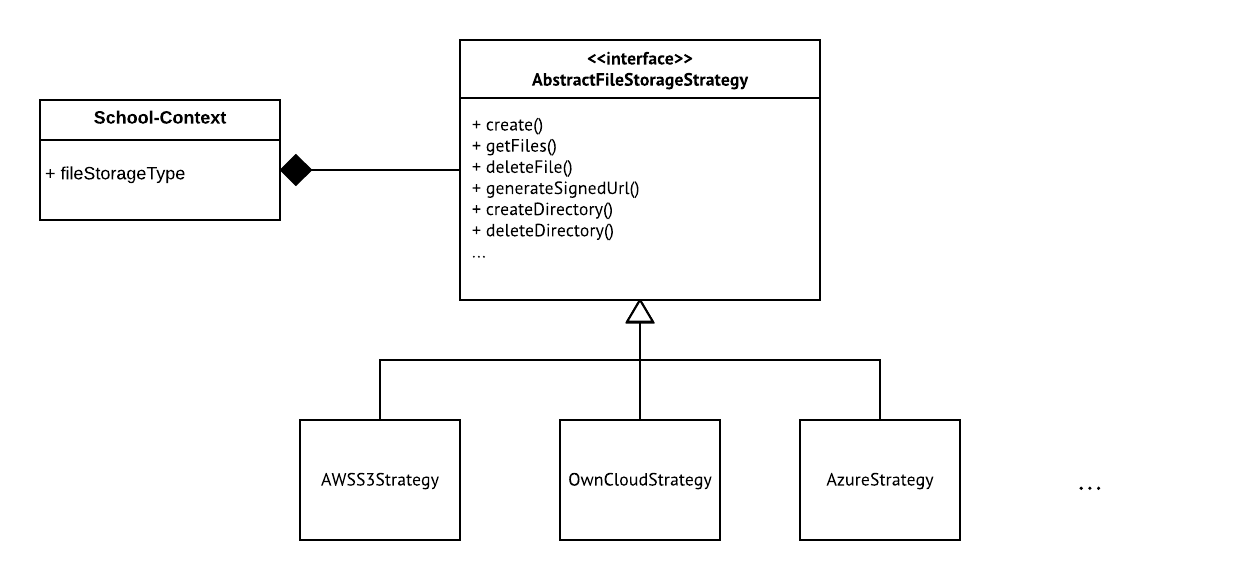
\includegraphics[width=1\linewidth]{images/strategypattern}
	\caption[Caption for concept]{Verteilung der Schul-Buckets mithilfe des Strategy-Patterns}
	\label{fig:strategy}
\end{figure}

\subsection{Interaktion verschiedener Schul-Cloud Komponenten}
\label{sec:interactionconcept}

Im Folgenden wird die Interaktion der verschiedenen Schul-Cloud Komponenten mithilfe von Beispielen beschrieben. Es wird stets von drei Rollen der Kommunikation geredet. Zum einen sorgt der \textit{Client} für die Nutzeraktion und steht somit für das Schul-Cloud Frontend, aber auch für eine mobile App. Der \textit{Server} meint den Schul-Cloud Server und dient als einer Art Proxy zu den verschiedenen File-Storage Providern. Dieser wird im Folgenden als \textit{Provider} bezeichnet. Als erstes Beispiel soll das Holen der persönlichen Dateien dienen. Abbildung \ref{fig:interacton_getFiles} zeigt die Interaktion der drei Komponenten. Der Client beginnt hierbei mit einem GET-HTTP-Request an die \textit{/fileStorage/} - Route vom Server. Um Dateien für einen bestimmten Kontext zu bekommen, muss im Query-Parameter \textit{path} der richtige Pfad mitgegeben werden. Für die persönlichen Dateien des Nutzers mit der ID \textit{123} ist dies \textit{users/123}. Man sieht hierbei die Rückführung auf den Grundaufbau der Dateiverwaltung. Die persönlichen Dateien eines jeden Schul-Cloud Nutzers werden im \textit{users} Unterordner der zugehörigen Schule gespeichert. Der ID-Ordner referenziert hier die Dateien des gesuchten Nutzers mit der ID \textit{123}. Dies muss eine valide Nutzer-ID sein, welche in der Schul-Cloud Datenbank gespeichert wird. Der Server kümmert sich nun um die Berechtigung, in dem er zum einen prüft, ob der im Client angemeldete Nutzer auch auf den Pfad zugreifen darf. Im Detail wird dies noch im Abschnitt \ref{sec:permissionsimpl}. beschrieben. Der Server ermittelt die Schule des Nutzers und fragt dann beim richtigen Provider die gesuchten Dateien für den gegebenen Pfad an. Dieser gibt dann die Datei-Objekte aus, welche dann über den Server zum Client ausgegeben werden. Man sieht hier sehr gut, dass der Schul-Cloud Server eine verwaltende Rolle einnimmt, ohne die Dateien tatsächlich physisch zu speichern. Er sorgt vielmehr für die Verteilung der Requests an die richtigen File Storage Provider. Dafür nutzt er das zuvor dargestellte Strategy-Pattern, um für eine Schule den richtigen Bucket zu finden.

\begin{figure}[H]
	\centering
	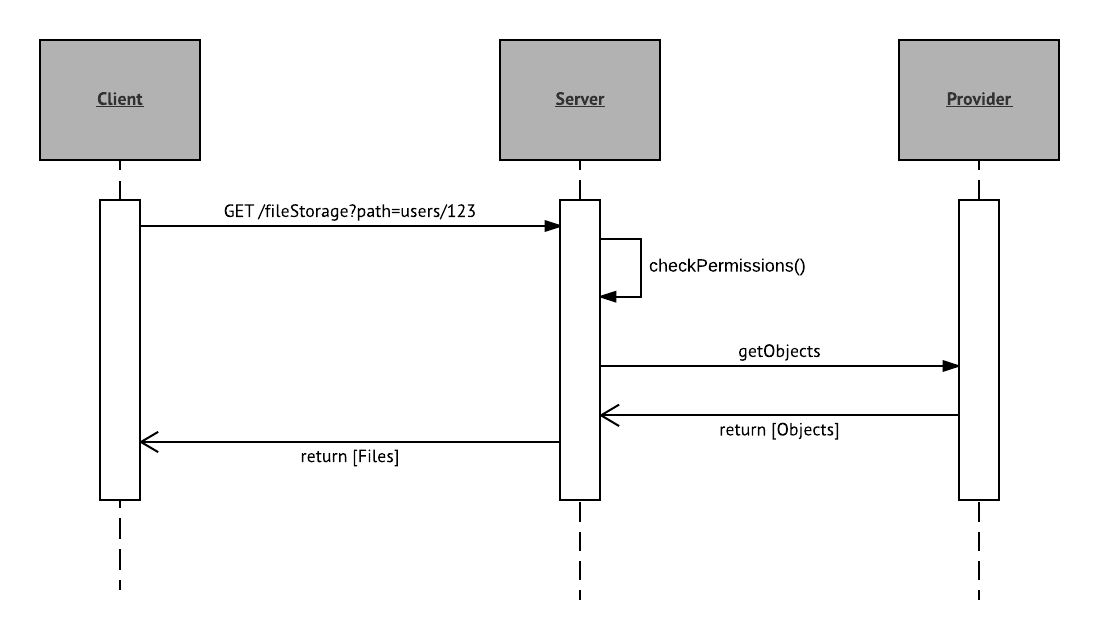
\includegraphics[width=1\linewidth]{images/fileumlsequence}
	\caption[Caption for concept]{Interaktion zwischen Client, Server und File Storage Provider  beim Holen von persönlichen Dateien}
	\label{fig:interacton_getFiles}
\end{figure}

Neben dieser einfachen dreigeteilten Interaktion zwischen Client, Server und Provider werden Upload und Download von Dateien direkt zwischen Client und Provider gehandhabt. Das hat den Grund, dass die Übertragung großer Datenmengen bei Dateien im Gigabyte - Bereich nicht über den Server laufen sollen. Abbildung \ref{fig:interaction_upload} zeigt dies anhand des Uploads einer Datei. Der Server fragt beim Provider nun eine Upload-URL an, auf welche der Client dann die Datei \textit{example.jpg} hochladen kann. Der Query-Parameter \textit{action} teilt mit, um welchen Typ von URL es sich handelt, im Falle von \textit{putObject} beim Upload einer Datei. Der Server prüft wieder die Berechtigungen des Clients und sendet dann die URL an den Client zusammen mit wichtigen Meta-Daten der Datei zurück. Diese soll der Client zusammen mit der Datei zum Provider laden, damit der Server später mehr Informationen über die Datei hat, zum Beispiel die Referenzierung eines Vorschaubilds.

\begin{figure}[H]
	\centering
	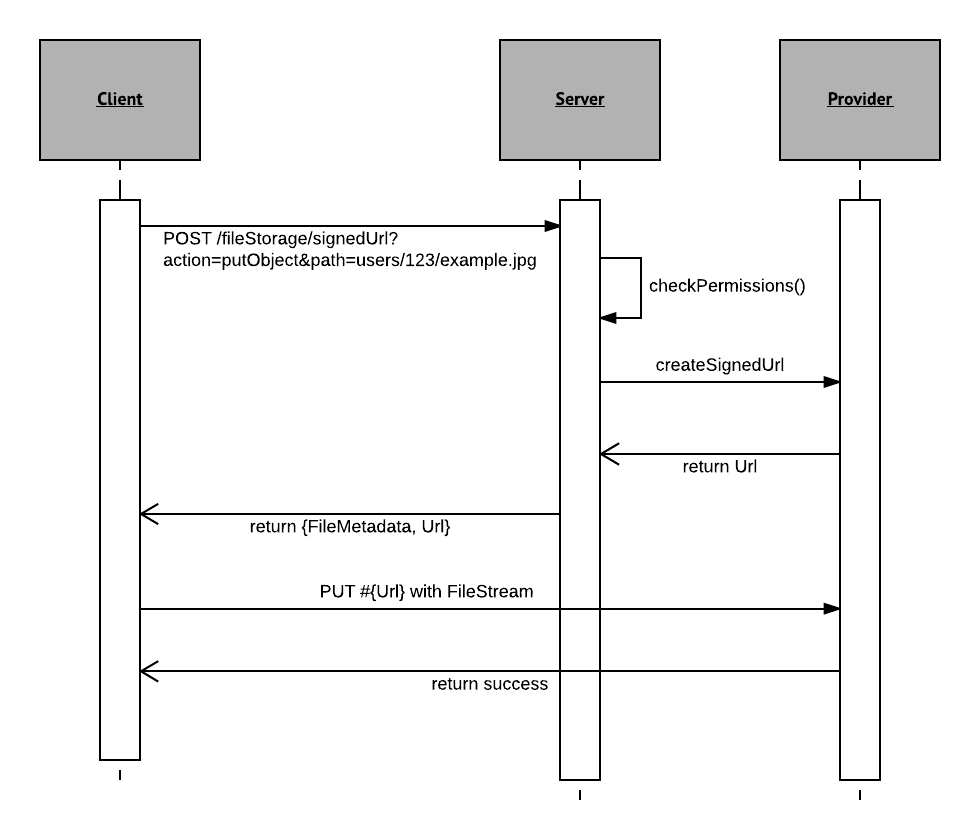
\includegraphics[width=1\linewidth]{images/fileuploadumlsequence}
	\caption[Caption for concept]{Interaktion zwischen Client, Server und File Storage Provider beim Upload einer Datei}
	\label{fig:interaction_upload}
\end{figure}


\subsection{Teilen von Dateien}
\label{sec:sharing_concept}

Zwar gibt der Aufbau der Dateiverwaltung eine klare Aufteilung zwischen Schul-, Kurs-, Fach - und Klassenkontexten vor, es soll jedoch trotzdem möglich sein, Dateien mit anderen Nutzern zu teilen. Das ist vor allem dann von Vorteil, wenn ein Lehrer eine persönliche Datei in seinem Unterricht direkt benutzen möchte. Zwar könnte der Lehrer dann die Datei in den jeweiligen Kursordner hochladen bzw. direkt im Unterrichtsmodus des Clients hochladen; welcher im Abschnitt \ref{sec:client} beschrieben wird; manchmal möchte der Lehrer trotzdem seine eigenen Dateien bei sich behalten und die Freigabe selbst steuern können. Ein weiteres Beispiel wäre es, wenn ein Schüler eine private Datei mit anderem teilen möchte, ohne sie im Kurskontext verfügbar zu machen. Somit muss es möglich sein, im Schul-Cloud Client einen Zugriffslink zu generieren. Dieses Prinzip findet auch bei ownCloud sowie Dropbox Einsatz und ist ein beliebter Weg, eigene Dateien schnell mit mehreren Personen zu  teilen. Abbildung \ref{fig:filesharinggeneration} zeigt den Prozess zur Generierung eines solchen Links für eine Datei. Der Client fordert die Freischaltung für das Teilen der Datei beim Server an. Dieser besteht intern aus dem eigentlichen File-Service und aus dem Link-Service, welcher als URL  Shortener \footnote{Kurz-URL-Dienst - \url{https://de.wikipedia.org/wiki/Kurz-URL-Dienst}} auftritt. Dieser dient dazu, den langen Link zu einer Schul-Cloud Datei etwas zu verkürzen und leichter teilbar zu machen. Nachdem der File-Service das Teilen freigegeben hat, fragt der Client einen solchen Shortlink an und gibt diesen im User Interface an. Dieser Prozess ist bekannt aus bereits bestehenden File Storage Providern.

\begin{figure}[H]
	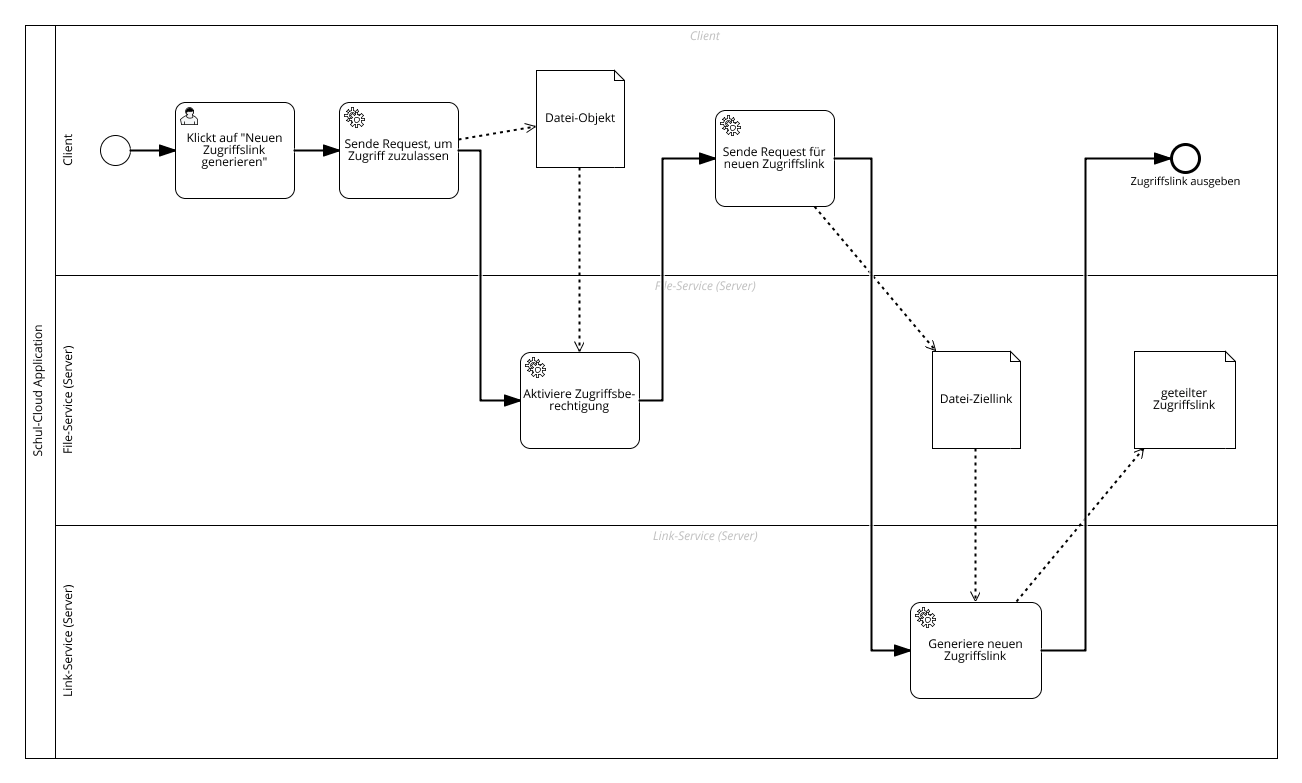
\includegraphics[width=1\linewidth]{images/filesharinggeneration}
	\caption[Caption for concept]{Generierung eines Zugriffslinks}
	\centering
	\label{fig:filesharinggeneration}
\end{figure}

Diesen Link kann der Besitzer der Datei nun an andere Schul-Cloud Nutzer weiterleiten. Den daraus resultierenden Zugriff ist in Abbildung \ref{fig:filesharingusing} (Anhang) modelliert. Der Client öffnet den Link und fragt zuerst beim Server an, ob die Sharing-Funktion für die Datei überhaupt freigeschaltet ist. Ist dies nicht freigegeben, erhält der Client einen Fehler. Im anderen Falle wird im Server gespeichert, welcher Nutzer auf die Datei zugreifen möchte, um den Prozess später zu beschleunigen und redundante Prüfungen zu verhindern. Außerdem können so für den Nutzer freigegebene Dateien zusammen aufgelistet werden, wie es Dropbox beispielsweise tut. Anschließend wird eine Anfrage auf die tatsächliche Datei über den Server an den Storage Provider gestellt und diese zurück an den Client gesendet. Dieser Teil des Prozesses ist sehr vereinfacht dargestellt, tatsächlich muss für das Holen der tatsächlichen Datei zunächst eine Zugriffs-URL, wie in Abschnitt \ref{sec:interactionconcept} beschrieben, generiert werden und an den Client geliefert werden.

\clearpage

	\section{Implementierung}
\label{sec:implementation}

Nachdem das grobe Konzept der Dateiverwaltung der Schul-Cloud geschildert wurde, werden anschließend Implementierungsdetails präsentiert. Diese wird in einer Zweiteilung erfolgen. Zunächst wird der relevante Code des Schul-Cloud Servers \footnote{Schul-Cloud Server - \url{https://github.com/schul-cloud/schulcloud-server}} aufgezeigt und beschrieben. Dann werden dazu passende Teile vom User Interface des Schul-Cloud Clients \footnote{Schul-Cloud Client - \url{https://github.com/schul-cloud/schulcloud-client}} dargelegt. Beide Komponenten sind öffentlich auf GitHub \footnote{GitHub - \url{https://github.com}} zugänglich.

\subsection{Schul-Cloud Server}
\subsubsection{Einbettung in das Schul-Cloud - Datenmodell}

Der Schul-Cloud Server basiert auf Node.js \footnote{Node.js - \url{https://nodejs.org}} und Feathers \footnote{Feathers - \url{https://feathersjs.com/}}, einer auf Express \footnote{Express - \url{http://expressjs.com/de/}} aufbauenden Schicht für das schnelle Entwickeln von REST-APIs \footnote{Representational State Transfer (REST) - \url{https://de.wikipedia.org/wiki/Representational_State_Transfer}}. Die Dateiverwaltung des Backends wird somit auch als typischer Feathers-Service bereitgestellt. Dieser befindet sich im Unterordner \textit{src/services/fileStorage} und beinhaltet die grundlegende Funktionalität der Dateiverwaltung. Anders als typische Feathers Services besitzt dieser kein MongoDB \footnote{MongoDB - \url{https://www.mongodb.com/de}} - Model, sondern dient eher als Proxy-Service. Die \textit{index.js} bündelt die drei Teilservices des File-Storage Services zusammen und macht sie nach außen zugänglich (Anhang \ref{code:filestorageindex}). Diese sind zum einem der \textit{FileStorageService}, welcher sich um die eigentliche Verteilung von Dateianfragen, wie das Erstellen und Löschen von Dateien, kümmert. Dazu kommt der \textit{SignedUrlService}, welcher die Zugriffslinks generiert. Als drittes gibt es den \textit{DirectoryService}, welcher zusätzliche Funktionalitäten für Ordner bereit stellt. Alle API-Routen werden unter \textit{/fileStorage/} registriert, wobei der \textit{SignedUrlService} unter \textit{/fileStorage/signedUrl} und der \textit{DirectoryService} unter \textit{/fileStorage/directories} verfügbar ist. Die einzelnen Beschreibungen aller API-Routen sind in der Dokumentation des Servers \cite{online:serverswagger} verfügbar. \\

In der \textit{index.js} des FileStorage Services erfolgt außerdem die Auswahl der richtigen Strategie für die Schule des Zugreifenden auf die API. Eine in der Schul-Cloud vermerkte Schule kann genau einen \textit{fileStorageType} besitzen, wie die \textit{model.js} des SchoolServices (\textit{src/services/school}) des Backends zeigt:

\begin{lstlisting}[label= schoolModel]
	'use strict';

	const fileStorageTypes = ['awsS3']; // aktuell unterstützte Strategien
	
	const schoolSchema = new Schema({
		name: {type: String, required: true},
		address: {type: Object},
		fileStorageType: {type: String, enum: fileStorageTypes}, // Eigenschaft zur Auswahl der richtigen Strategie
		systems: [{type: Schema.Types.ObjectId, ref: 'system'}],
		federalState: {type: Schema.Types.ObjectId, ref: 'federalstate'},
		createdAt: {type: Date, 'default': Date.now},
		updatedAt: {type: Date, 'default': Date.now}
	}	,{
		timestamps: true
	});
\end{lstlisting}

Vor dem Aufrufen jeder Route wird die Funktion \textit{resolveStorageType} in \textit{src/services/fileStorage/hooks/index.js} ausgeführt, die dafür sorgt, dass der Typ des Schul-Buckets aus der im Nutzer referenzierten Schule erhalten wird. Die \textit{userId} wird vorher wie bei Feathers üblich aus dem Request via Authentifizierung ermittelt.

\begin{lstlisting}[label= resolveStorageType]
	const resolveStorageType = (hook) => {
		let userService = hook.app.service("users");
		
		// finde angemeldeten Nutzer
		return userService.find({query: {
				_id: hook.params.payload.userId,
				$populate: ['schoolId'] // hole referenzierte Schule
			}}).then(res => {
			
				// speichere korrekten Typ
				hook.params.payload.fileStorageType = res.data[0].schoolId.fileStorageType;
				return hook;
		});
	};
\end{lstlisting}

Aus dieser Information kann der FileStorage Service dann die richtige Strategie wählen. Hier ein Beispiel für die Funktion \textit{find}, welche auf \textit{GET /fileStorage/} registriert ist und die Dateien für einen gegebenen Pfad holt:

\begin{lstlisting}[label=findFiles]
	/**
	* @returns {Promise}
	* @param query contains the file path
	* @param payload contains fileStorageType and userId, set by middleware
	*/
	find({query, payload}) {
		return createCorrectStrategy(payload.fileStorageType).getFiles(payload.userId, query.path);
	}
\end{lstlisting}

Die Funktion \textit{createCorrectStrategy} erzeugt ein Objekt für die jeweilige Strategie, welche in \textit{src/services/fileStorage/strategies} implementiert ist:

\begin{lstlisting}
	const strategies = {
		awsS3: AWSStrategy
	};

	const createCorrectStrategy = (fileStorageType) => {
		const strategy = strategies[fileStorageType];
		if (!strategy) throw new errors.BadRequest("No file storage provided for this school");
		return new strategy();
	};
\end{lstlisting}

\subsubsection{AWS S3 - Strategy als Beispiel}
\label{sec:awss3impl}

Im Schul-Cloud Server lassen sich eine Reihe von Strategien für verschiedene Typen von File Storage Providern implementieren. Diese werden im Ordner \textit{src/services/fileStorage/strategies} abgelegt. Die Klasse \textit{AbstractFileStorageStrategy} (Anhang \ref{code:strategyinterface}) gibt die zu implementierenden Funktionen vor. Die einzelnen Strategien sind somit Unterklassen dieser. In diesem Abschnitt wird die Implementierung für einen AWS S3-Adapter beschrieben. S3 dient während der Pilotphase der Schul-Cloud als Standart-Provider. Um schnell entwickeln zu können, wurde ein S3-Abbild auf dem Development-System der Schul-Cloud \footnote{Development-System - \url{https://schul.tech/}} eingestellt. Hierbei wurde \textit{minion} \footnote{minion - \url{https://github.com/minio/minio}} genutzt, einem Open Source Projekt, welches S3-API kompatible Funktionen bereitstellt. Die AWS S3-Strategy befindet sich in \textit{src/services/fileStorage/strategies/awsS3.js}. \\

Um Zugriff auf eine S3-Instanz zu bekommen, braucht die Strategie eine AWS-S3-Konfiguration. Das Node-Modul \textit{aws-sdk} \footnote{aws-sdk - \url{https://aws.amazon.com/de/sdk-for-node-js/}} bietet hierbei eine komplette Anbindungsmöglichkeit. Eine mögliche S3-Konfiguration könnte folgendermaßen aussehen:

\begin{lstlisting}
	
	const awsConfig =  {
		"signatureVersion": "v4",
		"s3ForcePathStyle": true,
		"sslEnabled": true,
		"accessKeyId": "password",
		"secretAccessKey": "password",
		"region": "eu-west-1",
		"endpointUrl": "http://localhost:3000"
	}
\end{lstlisting}

Mithilfe dieser Konfiguration und dem aws-sdk kann man nun Befehle an eine S3-Instanz schicken. Der AWS S3-Standard unterstützt alle die in der \textit{AbstractFileStorageStrategy} geforderten Funktionen. Im Anhang \ref{code:awsS3deletefile} wird die Implementierung der Funktion \textit{deleteFile} für das Löschen einer Datei in einem S3-Bucket gezeigt. In jeder Funktion der Strategie muss zuerst die Berechtigung geprüft werden. Dies übernimmt der \textit{filePermissionHelper}, welcher im nächsten Abschnitt näher vorgestellt wird. Ein weiterer wichtiger Punkt beim Verbinden mit der S3-Instanz ist das Erstellen eines AWS S3-Verbindungsobjekts (Zeile 13). Dieser beinhaltet die vorher angelegte Konfiguration sowie die Information, mit welchem Bucket sich verbunden werden soll. Da die Architektur vorgibt, dass Buckets zu Schulen gehören, ergibt sich der Name des Buckets einfach aus \textit{"bucket-" + schoolId}. Die Funktion \textit{createAWSObject} zeigt die Generierung dieses Objekts:

\begin{lstlisting}
	const createAWSObject = (schoolId) => {
		if (!awsConfig.endpointUrl) throw new Error('AWS integration is not configured on the server');
		
		// Verbinden der Konfiguration
		var config = new aws.Config(awsConfig);
		
		// Einstellen des S3-Endpunktes
		config.endpoint = new aws.Endpoint(awsConfig.endpointUrl);
		
		// Einstellen des gesuchten S3-Buckets
		let bucketName = `bucket-${schoolId}`;
		
		// Erstellen des S3-Objekts
		var s3 = new aws.S3(config);
		
		return { s3: s3, bucket: bucketName };
	};
\end{lstlisting}

In der Variable \textit{params} in Zeile 16 vom Anhang \ref{code:awsS3deletefile} wird dann angegeben, um welche Art von Aktion es sich auf das Bucket handelt. Da in dieser Funktion die mit \textit{path} angegebene Datei gelöscht werden soll, wird ein Array von zu löschenden Datei-Keys angelegt, welches die gesuchte Datei enthält. Eine S3-Datei ist immer über ihren Pfad referenziert. Es ist so theoretisch möglich, mehrere Dateien auf einmal zu löschen. Das macht sich die S3-Strategie beim Löschen von Ordnern zunutze. Zum Schluss wird die Aktion auf dem Bucket ausgeführt. Dafür wird üblicherweise \textit{awsObjekt.s3.deleteObjects(params)} genutzt. Um besser mit \textit{Promises} \footnote{Promises - \url{https://developer.mozilla.org/de/docs/Web/JavaScript/Reference/Global_Objects/Promise}} arbeiten zu können, wird \textit{promisify} \footnote{es6-promisify - \url{https://www.npmjs.com/package/es6-promisify}} um die Funktion gelegt. Der Vorteil des Strategy-Patterns ist es nun, dass die Anbindung an eine ownCloud-Instanz komplett anders implementiert werden kann. Man muss nur darauf achten, dass Ein- und Ausgabe-Parameter gleich sind. Hier macht sich der Status als Open Source Projekt bezahlt, da externe Entwickler verschiedene Strategien mit einbringen und so den File-Storage Service der Schul-Cloud beliebig erweitern können. Die S3-Strategie bietet hier einen sehr guten Einstiegspunkt für weitere Implementierungen.

\subsubsection{Berechtigungsverwaltung}
\label{sec:permissionsimpl}

Vor jedem Aufruf einer Dateioperation werden die Berechtigungen des zugreifenden Nutzers geprüft. Wie im Anhang \ref{code:awsS3deletefile} (Zeile 5) zu sehen ist, kümmert sich der \textit{filePermissionHelper} darum. Dieser befindet sich in \textit{src/services/filePermission/utils/filePermissionHelper.js} und gehört zum \textit{FilePermissionService}, einem weiteren Feathers Service, der sich ausschließlich um die Rechteverwaltung innerhalb der Dateiverwaltung kümmert. Die Funktion \textit{checkPermissions()} ist folgendermaßen aufgebaut:

\begin{lstlisting}
	checkPermissions(userId, filePath, permissions = ["can-read", "can-write"]) {
		return this.checkNormalPermissions(userId, filePath)
			.catch(err => this.checkExtraPermissions(userId, filePath, permissions));
	}
\end{lstlisting}

Wie hier zu sehen, teilt sich die Überprüfung in zwei einzelne Berechtigungschecks. Zum einen wird in der Funktion \textit{checkNormalPermissions} die generelle Berechtigung überprüft, etwa ob es sich um eine eigene Datei handelt bzw. um eine Kursdatei und der zugreifende Nutzer Teilnehmer dieses Kurses ist. Diese Informationen erhält er aus dem \textit{filePath}, da in diesem die Zugehörigkeit der Datei enthalten ist (siehe Abschnitt \ref{sec:basicaufbau}). Die komplette Implementierung dieses Checks findet sich im Anhang \ref{code:fphnormal}. Sollte diese Überprüfung fehlschlagen, gibt es noch die Möglichkeit, dass der Zugreifende die Datei von einem anderen Nutzer freigegeben bekommen hat. Dann muss ein Datenbankeintrag vom Typ \textit{FilePermissionModel} für den Nutzer und die Datei existieren. Der \textit{FilePermissionService} verwaltet dieses Datenbankmodell in der Datei \textit{src/services/filePermission/model.js}:

\begin{lstlisting}
	const permissionTypes = ['can-read', 'can-write'];
	
	const filePermissionSchema = new Schema({
		key: {type: String, required: true, unique : true},
		permissions: [{
			userId: {type: Schema.Types.ObjectId, ref: 'user'},
			permissions: [{type: String, enum: permissionTypes}]
		}],
		createdAt: {type: Date, 'default': Date.now},
		updatedAt: {type: Date, 'default': Date.now}
	});
\end{lstlisting}

Um eine zusätzliche Zugriffsberechtigung auf die Datei zu bekommen, muss ein solcher Eintrag in der Datenbank existieren. Die Eigenschaft \textit{key} beinhaltet den Pfad der Datei. Im Array \textit{permissions} sammeln sich Tupel aus Nutzer-ID und bestimmten Rechten. Das können Schreib- sowie Leserechte sein. Um die Menge an Datenbankeinträgen zu sparen, gibt es für jede Schul-Cloud Datei nur einen Eintrag, welche alle zusätzlichen Berechtigungen in \textit{permissions} speichert. Somit kann man zum Beispiel überprüfen, ob eine Datei für einen bestimmten Nutzer zum Teilen freigegeben wurde. Falls es für eine Datei ein Datenbankeintrag mit einem leeren \textit{permissions} Array existiert, gibt dies schon Auskunft darüber, ob die Datei überhaupt zum Teilen freigegeben ist, zum Beispiel wenn ein geteilter Link im Client erstellt wurde. Momentan ist nur die Freigabe für einzelne Nutzer möglich, so dass man bei Gruppenfreigaben jeden einzelnen Benutzer hinzufügen müsste. Dies lässt sich aber noch auf Gruppenebene erweitern. Mit diesen Datenbankeinträgen überprüft die Funktion \textit{checkExtraPermissions()} (Anhang \ref{code:fphextra}), ob eine zusätzliche Zugriffsberechtigung für den Nutzer und der gegebenen Datei existiert. Führen beide Checks zu keinem positiven Ergebnis, hat der Nutzer definitiv keine Berechtigung für diese Datei.

\subsection{Schul-Cloud Client}
\label{sec:client}

\subsubsection{Anbindung zum Server}
Der Schul-Cloud Client ist ebenfalls mit Node.js implementiert. Er kommt ohne großes Web-Framework aus und basiert auf einem einfachen Express-Server. Hier benutzt er \textit{Handlebars} \footnote{Handlebars - \url{http://handlebarsjs.com/}} als Template Engine. Die Anbindung an den Schul-Cloud Server erfolgt über den \textit{filesController} in der  Datei \textit{controllers/files.js}. Hier gibt es eine Reihe von Dateioperationen, welche regelmäßig mit dem Schul-Cloud Server interagieren. Ein Beispiel ist das Erstellen eines neuen Ordners:

\begin{lstlisting}
	// erstelle neuen Ordner
	router.post('/directory', function (req, res, next) {
		const {name, dir} = req.body;
	
		const basePath = dir;
		const dirName = name || 'Neuer Ordner';
		
		// Server-Anbindung
		api(req).post('/fileStorage/directories', {
			json: {
				path: basePath + dirName,
			}
		}).then(_ => {
			
			// Rückmeldung an den Browser
			res.sendStatus(200);
		}).catch(err => {
			res.status((err.statusCode || 500)).send(err);
		});
	});
\end{lstlisting} 

Für jeden Zugriff auf den Server dient das \textit{api} - Objekt, welches in der Datei \textit{api.js} im Stammverzeichnis initialisiert wird. Dieser baut eine einfache Verbindung zum Schul-Cloud Server auf und macht HTTP-Requests möglich. Zum Erstellen eines Ordners muss man demzufolge \textit{POST /fileStorage/directories/} aufrufen. Der \textit{filesController} sorgt zudem für das Rendering der richtigen Template-Dateien.

\subsubsection{User Interface}
\label{sec:userinterface}
Im Folgenden wird auf die genaue Implementierung der einzelnen Dateioperationen im Client nicht näher eingegangen. Viel mehr liegt der Schwerpunkt auf die Nutzerinteraktion. Dazu dienen einzelne Screenshots vom Schul-Cloud Produktivsystem \footnote{Schul-Cloud Produktivsystem - \url{https://schul-cloud.org}} (Stand \today). Die Projektstruktur gibt vor, dass sich das User Interface der Dateiverwaltung im Unterordner \textit{views/files} befindet. Die normale Dateiverwaltung befindet sich auf der Route \textit{/files/} bzw. unter dem Menüpunkt "Meine Dateien". Hier sieht man zunächst die persönlichen Dateien (Anhang Abbildung \ref{fig:screenMeineDateien}), d.h. alle diejenigen, die unter \textit{"users/" + Nutzer-ID} des angemeldeten Nutzers gespeichert sind. In der Seitennavigation sieht man nun weitere Menüpunkte unter "Meine Dateien". So kann man nun auf die Kurs- sowie Klassendateien zugreifen. In dieser Dateiverwaltung hat man außerdem die Möglichkeit, die Datei im Browser zu öffnen. Ähnliche Funktionalitäten enthalten außerdem die Android \footnote{Schul-Cloud Android-App - \url{https://github.com/schul-cloud/schulcloud-mobile-android}} - und iOS \footnote{Schul-Cloud iOS-App - \url{https://github.com/schul-cloud/schulcloud-mobile-ios}} - App der Schul-Cloud.

Neben der normalen Dateiansicht für persönliche, Kurs - und Klassendateien hat man außerdem die Möglichkeit, als Lehrer Dateien direkt im Unterrichtskontext einzufügen. Dazu geht man auf einen Kurs, dann auf ein Thema, bearbeitet dieses Thema und fügt eine Text-Komponente hinzu. Hier wurde der eingebaute \textit{ckEditor} \footnote{ckEditor - \url{http://ckeditor.com/}} so überarbeitet, dass man entweder per Drag \& Drop eine Datei hineinschieben oder über die Bilderauswahl ein Bild aus dem Kurskontext auswählen kann (Anhang Abbildung \ref{fig:screenCkEditor}). So hat man die Möglichkeit, Bilder als Lernelemente im Themeneditor einzubinden (Anhang Abbildung \ref{fig:screenTopicEditor}).

\subsubsection{Administration}

Da es einer Schule möglich sein soll, selbst über die Art des File Storage Providers zu bestimmen, gibt es für die Rolle \textit{Administrator} einen besonderen Menü-Punkt in der Seitenmenüleiste. Unter ``Administration" kann der Administrator einer Schule neben anderen Informationen auch den File Storage Typ auswählen (Anhang Abbildung \ref{fig:adminFileStorage}). Hier soll es in Zukunft auch ein Import für bestehende Dateiablagen sowie die Einstellung für Berechtigungen geben.

\subsubsection{Dateien teilen}

Das Teilen von Dateien funktioniert wie in Abschnitt \ref{sec:sharing_concept} beschrieben momentan mit dem Generieren von Zugriffslinks. Dafür kann man auf das Teilen-Icon an einer Datei klicken und ein Modal-Fenster mit einem neuen Link öffnet sich (Anhang Abbildung \ref{fig:sharingfileui}). Dieser kann an mehrere Leute weitergegeben werden. Erst mit dem Klick auf das Teilen-Icon wird die Teilen-Funktion freigeschaltet. 

\clearpage

	\section{Evaluierung}
\label{sec:evaluation}

\clearpage

	\section{Future Work}
\label{sec:futurework}

\clearpage

	\section{Zusammenfassung}
\label{sec:conclusion}

Eines der übergeordneten Ziele der deutschen Schul-Cloud ist es, Lernmaterial für alle und überall zugänglich zu machen. Diese Arbeit wollte erreichen, eine flexible Dateiverwaltung für dieses Vorhaben zu entwerfen und zu implementieren. Die Anforderungen wurden zu Beginn des Projekts klar definiert, so dass das Konzept auf diesen aufbauen konnte.

 Es wurde sich für ein in Schulen aufgeteiltes Bucket-System entschieden, um Dateien logisch zu trennen. Diese werden in die einzelnen Kontexte des schulischen Alltags untergliedert, d.h. Kurse bzw. Fächer sowie Klassen und einzelne Individuen. Das Strategy-Pattern schaffte zudem die Möglichkeit, Buckets auf mehrere Server zu verteilen. Das Ziel einer grundlegend verteilten Dateiverwaltung wurde somit erfüllt. Viele Konzepte für die Dateiverwaltung wurden vom AWS S3-Standard abgeleitet. Da viele anderen Systeme wie zum Beispiel Microsoft Azure \footnote{Microsoft Azure - \url{https://azure.microsoft.com/de-de/}} auf den Standard aufbauen, liegt es nahe, diesen im Schul-Cloud System zu benutzen. Das Strategy-Pattern ermöglicht es trotzdem, von diesem abzuweichen und ganz eigene Strategien zu implementieren.

Der Open-Source Status der Schul-Cloud soll hierbei helfen, zusammen mit Schülern und Lehrern die Schul-Cloud weiter zu verbessern. Strategien können nach und nach dazu implementiert werden und ins bestehende System eingepflegt werden. Eine Schule hat so zum Beispiel die Möglichkeit, für ihren Schul-Server eine eigene Anbindung zu schreiben, ohne sich zu stark an den Schul-Cloud Standard zu richten. Abschließend lässt sich sagen, dass die entworfenen Konzepte in der derzeit laufenden Pilotphase getestet und Rückmeldungen eingeholt werden müssen.

\clearpage


	%%% Bibliography
	%\bibliographystyle{babunsrt3-fl}
	\addcontentsline{toc}{section}{Literatur}
	\bibliographystyle{gerplain}
	\bibliography{projektbib}
	\clearpage

	%%%% Appendix
	\appendix
\section{Appendix}
\label{sec:appendix}

\begin{lstlisting}[caption=Abstract file storage strategy, label=strategyinterface]
class AbstractFileStorageStrategy {
	constructor() {
		if (new.target === AbstractFileStorageStrategy) {
			throw new TypeError("Cannot construct AbstractFileStorageStrategy instances directly.");
		}
	}
	
	create() {
		throw new TypeError("create method has to be implemented.");
	}
	
	getFiles() {
		throw new TypeError("getFiles method has to be implemented.");
	}
	
	deleteFile() {
		throw new TypeError("deleteFile method has to be implemented.");
	}
	
	generateSignedUrl() {
		throw new TypeError("generateSignedUrl method has to be implemented.");
	}
	
	createDirectory() {
		throw new TypeError("createDirectory method has to be implemented.");
	}
	
	deleteDirectory() {
		throw new TypeError("deleteDirectory method has to be implemented.");
	}
}

module.exports = AbstractFileStorageStrategy;
\end{lstlisting}

\clearpage

	%%% TODOs
	%\todo[inline]{The original todo note withouth changed colours.\newline Here's another line.}
	%\lipsum[1]\unsure{Is this correct?}\unsure{I'm unsure about also!}
	%\lipsum[1]\change{Transate abstract}
	%\lipsum[1]\info{This can help me in chapter seven!}
	%\lipsum[1]\improvement{This really needs to be improved!\newline\newline What was I thinking?!}
	%\thiswillnotshow{This is hidden since option `disable' is chosen!}
	%\improvement[inline]{The following section needs to be rewritten!}
	%\listoftodos[Notes]

\end{document}
